\subsection{Introduzione}

Il framework \textsl{JSF} (acronimo per \textsl{Java Server Faces}) fa parte delle tecnologie standard della piattaforma \textsl{Java EE} e il suo scopo è quello di facilitare lo sviluppo dell'interfaccia utente di un'applicazione web. È un framework \textit{component-based}: consente allo sviluppatore di costruire una pagina web focalizzandosi sugli oggetti che la compongono, piuttosto che sul codice HTML che la genera, permettendo pertanto un livello di astrazione maggiore. \\
Ne esistono diverse implementazioni; nello sviluppo della applicazione è stata utilizzata quella di riferimento, \textsl{Mojarra} (versione 2.1), nonché la libreria \textsl{PrimeFaces} (versione 3.5) per estenderne le funzionalità.\\
Nei prossimi paragrafi si esamineranno un po' più in dettaglio le caratteristiche ed il funzionamento di JSF.


\subsection{Caratteristiche}

\subsubsection{Panoramica}

La tecnologia JSF è composta essenzialmente da due componenti:

\begin{itemize}
\item Un insieme di API che consentono di:
\begin{itemize}
\item rappresentare ed utilizzare i componenti
\item gestire gli eventi
\item effettuare la conversione dei dati
\item eseguire una validazione lato server dei dati
\item definire le regole di navigazione fra le pagine
\item creare applicazioni multi-lingua
\end{itemize}
\item Librerie per la gestione dei tag e la connessione dei componenti ad oggetti Java lato server.
\end{itemize}

Inoltre, la struttura del framework è tale da consentire l'estensione delle funzionalità e l'aggiunta di nuovi componenti.\\

\subsubsection{Architettura del framework}

\begin{figure}
	\centering
	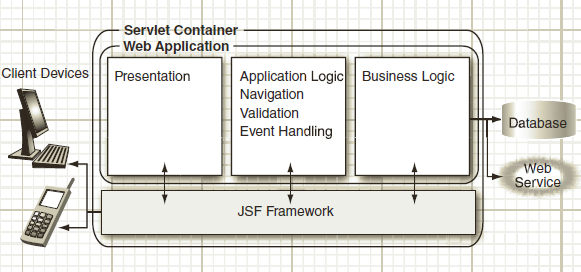
\includegraphics{JSF_architecture.png}
	\caption{Architettura di JSF}
	\label{jsf_arch}
\end{figure}

L'architettura di JSF (illustrata in Figura \ref{jsf_arch} ) segue il classico schema \textit{Model-View-Controller}: JSF consente di collegare il modello (\textit{model}) con l'interfaccia grafica (\textit{view}), fornendo gli strumenti necessari per poter controllare e processare le azioni degli utenti e aggiornare il modello sottostante di conseguenza (\textit{controller}). Tali strumenti realizzano principalmente tre tipi di servizi:

\begin{itemize}
\item \textbf{gestione degli eventi}: interagendo con la pagina web, l'utente può compiere una grande varietà di azioni; esse vengono rilevate dal browser, che \textquoteleft lancia\textquoteright{} il relativo evento. JSF consente di elaborare la risposta del programma tramite un meccanismo molto semplice: è possibile associare ad un dato evento un metodo di un oggetto Java lato server che si occupa della sua gestione.
\item \textbf{conversione dei dati}: nel web, i dati vengono immessi, visualizzati e scambiati sotto forma di stringa; il modello dei dati, invece, è composto da oggetti Java. JSF permette in modo agevole di effettuare le conversioni necessarie per consentire l'interazione tra questi due mondi: oltre a fornire dei convertitori per i tipi basilari (come ad esempio numeri o stringhe), offre anche la possibilità di definire convertitori personalizzati.
\item \textbf{validazione dei dati}: viene realizzata in modo simile alla conversione: lo sviluppatore può decidere di utilizzare i \textit{validator} standard o implementarne di nuovi. Tramite questo meccanismo si evita che gli errori dell'utente pregiudichino la validità del modello.
\end{itemize}


\subsubsection{Bean}

Il livello \textit{controller} di JSF fa un uso intensivo dei \textsl{bean}. Un bean è un oggetto Java gestito dal framework e non in maniera diretta dal programmatore.\\
Esistono vari tipi di bean; quelli a cui si può accedere direttamente da una pagina JSF sono detti \textit{managed bean}. Per essere tale, un bean deve avere un nome ed uno \textit{scope}, ossia un contesto in cui il bean è \textquoteleft visibile\textquoteright{} ed utilizzabile dall'applicazione. \\
Per maggiori dettagli, si rimanda al capitolo \ref{cdi}.


\subsection{Funzionamento}

\subsubsection{\textit{Rendering} delle pagine}
Ci sono diversi modi per creare una pagina JSF. Quello standard fa uso della tecnologia \textsl{Facelets}, che è stata sviluppata proprio per essere utilizzata da JSF; per creare una pagina Facelets è infatti sufficiente scrivere un documento XHTML che fa uso dei tag di JSF, con la possibilità di utilizzare l'\textsl{Expression Language} (\textsl{EL}) per consentire la comunicazione tra il livello presentazione e il livello applicazione. Ciascun tag è associato ad una classe che lo gestisce e le istanze di queste classi sono dette \textit{tag handler}: quando la pagina viene letta, i \textit{tag handler} vengono eseguiti e costruiscono un albero dei componenti della pagina (\textit{component tree}). Ad ogni tag corrisponde un nodo dell'albero. Ogni componente è inoltre associato ad un oggetto \textit{renderer}, che produce codice HTML in relazione allo stato del componente stesso (processo che viene detto \textit{encoding}).\\
La pagina così prodotta arriva all'utente. Quando l'utente invia dati al server, questo processa la richiesta e produce una serie di coppie ID/valore che viene memorizzata in una tabella hash. Ciascun componente può quindi consultarla e stabilire quali sono i valori relativi al tag ad esso associato, salvandoli come \textsl{valori locali} (o \textit{local values}). Questa operazione è chiamata \textit{decoding}.\\

\begin{figure}
	\centering
	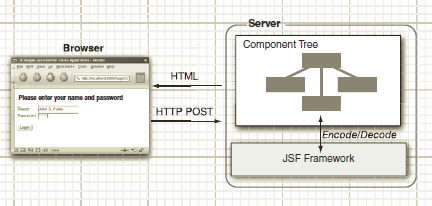
\includegraphics{JSF_client-server_communication.png}
	\caption{\textit{Encoding} e \textit{decoding}}
	\label{jsf_cs_comm}
\end{figure}

\subsubsection{\textit{Comunicazione client-server}}
La comunicazione tra client e server può avvenire essenzialmente in due modi, entrambi standard: tramite richieste \textsl{POST} e \textsl{GET}. JSF inoltre supporta nativamente ed in modo trasparente le richieste AJAX, consentendo di creare pagine web dinamiche. La comunicazione asincrona tramite AJAX è uno strumento molto efficace in vari contesti; la figura \ref{jsf_ajax} mostra come possa ad esempio essere utilizzata per la gestione degli eventi e la validazione dei dati.\\

\begin{figure}
	\centering
	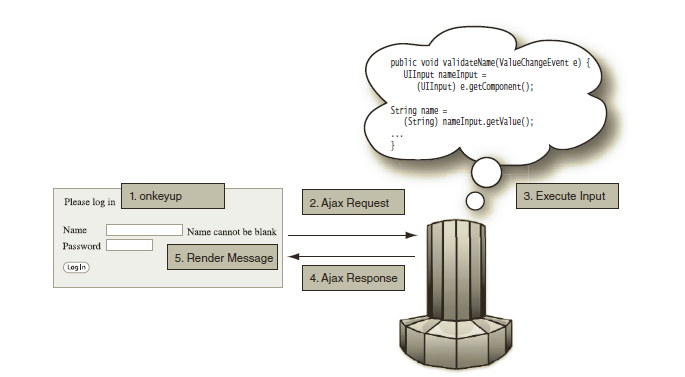
\includegraphics{JSF_ajax.png}
	\caption{Richiesta AJAX per la validazione di un input}
	\label{jsf_ajax}
\end{figure}

\subsubsection{\textit{Ciclo di vita}}
Ciò che viene eseguito tra una richiesta HTTP e la relativa risposta è chiamato dalla specifica JSF \textsl{ciclo di vita} (in inglese \textit{life cycle}).
Di seguito vengono riportate le sei fasi del ciclo di vita di JSF (raffigurate nella figura \ref{jsf_lifecycle}), come stabilito dalla specifica:

\begin{enumerate}
\item \textbf{\textit{Restore view}}: è la fase in cui viene costruito l'albero dei componenti, o viene recuperato nel caso di pagina mostrata precedentemente.
\item \textbf{\textit{Apply request values}}: in questa fase, la richiesta HTTP che l'utente invia al server viene processata, eseguendo l'operazione di \textit{decoding}.
\item \textbf{\textit{Process validations}}: viene eseguita la conversione e la validazione dei dati dell'utente.
\item \textbf{\textit{Update model values}}: durante questa fase viene aggiornato il modello dei dati.
\item \textbf{\textit{Invoke application}}: è la fase in cui il \textit{navigation handler} di JSF decide quale pagina visualizzare in base alle decisioni prese dal controllore.
\item \textbf{\textit{Render response}}: viene eseguito l'\textit{encoding}, producendo una pagina HTML che viene poi inviata al browser tramite la risposta del server.
\end{enumerate}

\begin{figure}
	\centering
	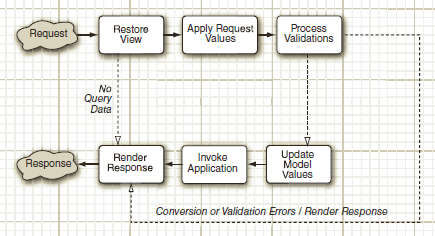
\includegraphics{JSF_life_cycle.png}
	\caption{Ciclo di vita di JSF}
	\label{jsf_lifecycle}
\end{figure}

Non sempre vengono eseguite tutte le fasi del ciclo di vita. Alcuni esempi:

\begin{itemize}
\item Nel caso in cui la richiesta HTTP non contenga valori, a seguito della fase \textit{Restore view} viene eseguita immediatamente la fase \textit{Render response}. Ciò accade, ad esempio, quando una pagina viene visualizzata per la prima volta.
\item Se si riscontrano errori di conversione o validazione durante la fase \textit{Process validations}, si passa alla fase \textit{Render response}: viene visualizzata nuovamente la stessa pagina, mostrando i relativi messaggi di errore (se previsti nella creazione della pagina stessa da parte dello sviluppatore).
\item In una richiesta AJAX vengono indicati quali componenti processare e quali aggiornare. Per i primi vengono eseguite le prime cinque fasi del ciclo di vita e successivamente viene eseguito il \textit{rendering} solo per i componenti da aggiornare.
\end{itemize}
















